\begin{frame}[<*>]{002班(电气)课程信息}
	\begin{itemize}
		\item 课时: 共$10$周$40$课时, 从 2025-09-09 到 2025-11-13
		\item 期末考试在课程结束后两周左右
	\end{itemize}
	\begin{twopart}{180pt}
		\begin{center}
			
\includegraphics[height=40mm]{../image/002.png}\\
			002班(电气)QQ群: \emph{\textbf{1002019981}}\\
			入群答案 \alert{\textbf{1400261B}}
		\end{center}
		\tcblower
		\begin{center}
			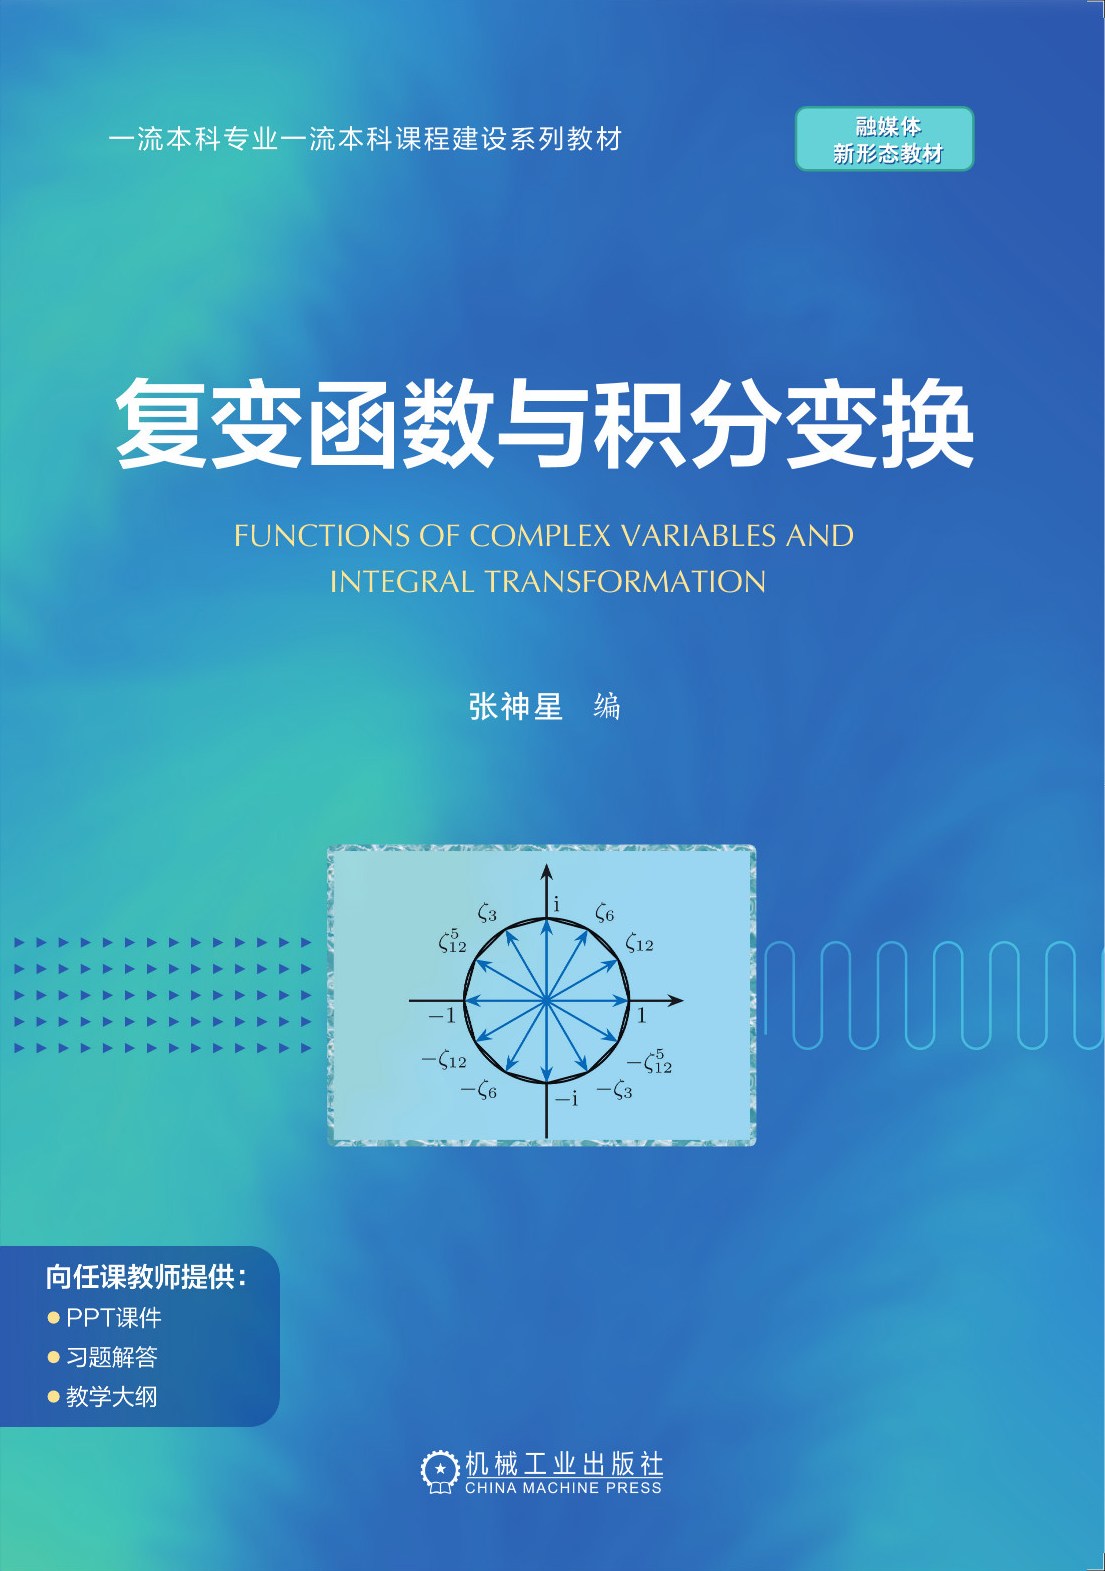
\includegraphics[height=40mm]{../image/book.png}\\
			教材: 《复变函数与积分变换》
		\end{center}
	\end{twopart}
\end{frame}


\begin{frame}[<*>]{003班(自动化)课程信息}
	\begin{itemize}
		\item 课时: 共$10$周$40$课时, 从 2025-09-09 到 2025-11-13
		\item 期末考试在课程结束后两周左右
	\end{itemize}
	\begin{twopart}{180pt}
		\begin{center}
			
\includegraphics[height=40mm]{../image/003.png}\\
			003班(自动化)QQ群: \emph{\textbf{1006453495}}\\
			入群答案 \alert{\textbf{1400261B}}
		\end{center}
		\tcblower
		\begin{center}
			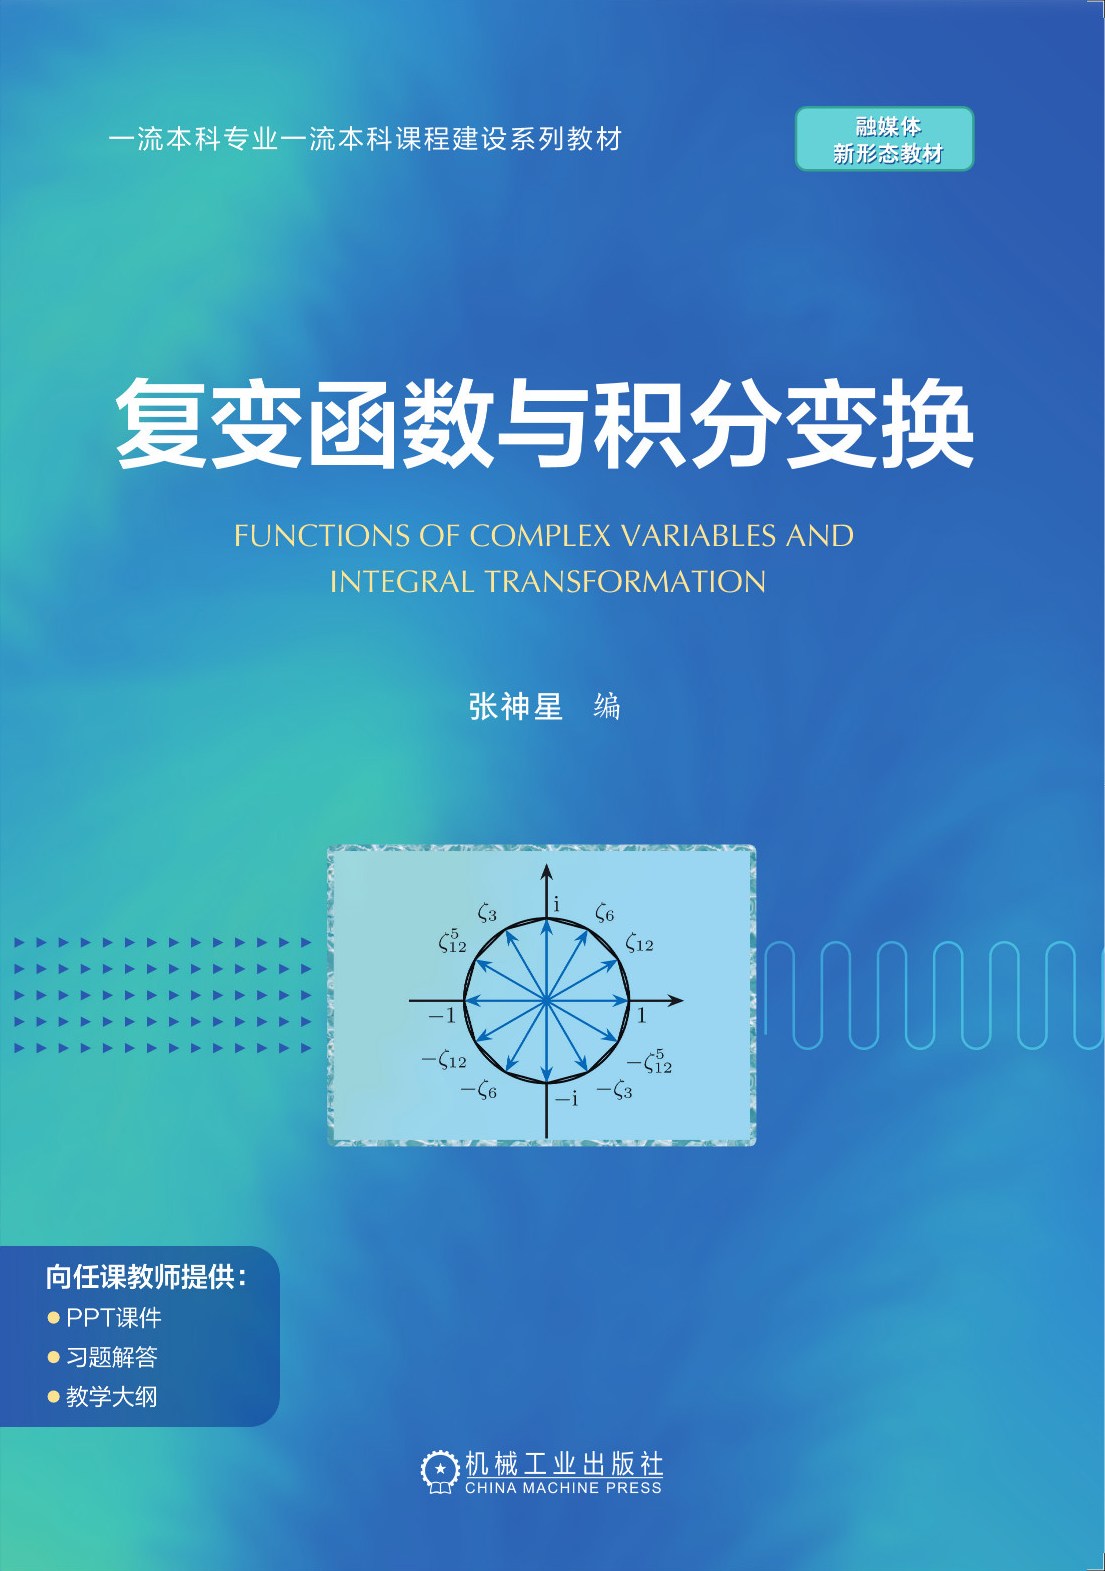
\includegraphics[height=40mm]{../image/book.png}\\
			教材: 《复变函数与积分变换》
		\end{center}
	\end{twopart}
\end{frame}


\begin{frame}{成绩构成}
	\bigdel
	\begin{center}
	\begin{tikzpicture}
		\begin{scope}
			\begin{scope}[xshift=.2mm,yshift=1.7mm,scale=2]
				\filldraw[cstcurve,main,cstfill1] (0,0)--(0,1) arc (90:144:1) -- cycle;
			\end{scope}
			\draw[main] (-.7,1.5)--(-1.6,2.5)--(-3,2.5);
			\filldraw[main,cstfill1] (-.7,1.5) circle(.1);
			\node at (-4.6,2) [text width=28mm]  (1){
				\begin{main}[
					title=作业 15分,
					centerbox,
					frame style={draw=none},
					borderline north={1pt}{-1pt}{main},
					borderline south={1pt}{-1pt}{main},
				]\kaishu
					作业通过超星发布和提交, 约两周交一次.
					\alert{作业必须按时提交, 不允许补交}.
				\end{main}
			};
		\end{scope}

		\begin{scope}
			\begin{scope}[xshift=1.5mm,yshift=1.7mm,scale=2]
				\filldraw[cstcurve,second,cstfill2] (0,0)--(1,0) arc (0:90:1) -- cycle;
			\end{scope}
			\draw[second] (.9,1.5)--(1.6,2.5)--(3,2.5);
			\filldraw[second,cstfill2] (.9,1.5) circle(.1);
			\node at (4.6,1.8) [text width=28mm] (2){
				\begin{second}[
					title=课堂测验 25分,
					centerbox,
					frame style={draw=none},
					borderline north={1pt}{-1pt}{second},
					borderline south={1pt}{-1pt}{second},
				]\kaishu
					课堂测验共3次, 取最高的两次平均. 测验范围和时间会提前通知. \alert{测验时在教室内作答,否则按未考处理}. 
				\end{second}
			};
		\end{scope}

		\begin{scope}
			\begin{scope}[xshift=1.8mm,yshift=.5mm,scale=1.95]
				\filldraw[cstcurve,third,cstfill3] (0,0)--({cos{36}},-sin{36}) arc (-36:0:1) -- cycle;
			\end{scope}
			\draw[third] (1.5,-.4)--(2.2,-1.1)--(3,-1.1);
			\filldraw[third,cstfill3] (1.5,-.4) circle(.1);
			\node at (4.6,-1.2) [text width=28mm] (3){
				\begin{third}[
					title=其它 10分,
					centerbox,
					frame style={draw=none},
					borderline north={1pt}{-1pt}{third},
					borderline south={1pt}{-1pt}{third},
				]\kaishu
					完成超星各个章节的任务点.
				\end{third}
			};
		\end{scope}

		\begin{scope}
			\begin{scope}[scale=2.1]
				\filldraw[cstcurve,fourth,cstfill4] (0,0)--({cos{144}},sin{144}) arc (144:324:1) -- cycle;
			\end{scope}
			\draw[fourth] (-.7,-1)--(-1.6,-1.7)--(-3,-1.7);
			\filldraw[fourth,cstfill4] (-.7,-1) circle(.1);
			\node at (-4.6,-1) [text width=28mm] (4){
				\begin{fourth}[
					title=期末考试 50分,
					centerbox,
					frame style={draw=none},
					borderline north={1pt}{-1pt}{fourth},
					borderline south={1pt}{-1pt}{fourth},
				]\kaishu
					期末卷面需要达到45分才计算总评分数, 45分以下直接不及格.
				\end{fourth}
			};
		\end{scope}
	\end{tikzpicture}
\end{center}
\end{frame}



\begin{frame}{复变函数的应用}
	\onslide<+->
	复变函数的应用非常广泛, 它包括:
	\begin{itemize}
		\item \alert{数学}中的代数、数论、几何、分析、动力系统……
		\item \alert{物理学}中流体力学、材料力学、电磁学、光学、量子力学……
		\item \alert{信息学}、\alert{电子学}、\alert{电气工程}……
	\end{itemize}
	\onslide<+->
	可以说复变函数应用之广, 在大学数学课程中仅次于高等数学和线性代数. 
\end{frame}


\begin{frame}{课程内容关系}
	\begin{center}
		\begin{tikzpicture}[node distance=18pt]
			\node[cstnode4] (1) {复数的要素};
			\node[cstnode4] (2) [right=35pt of 1] {四则运算};
			\node[cstnode4] (3) [right=32pt of 2] {幂和方根};
			
			\node[cstnode4] (11) [below=of 1] {数列极限};
			\node[cstnode4] (12) [below=of 2] {函数极限};
			\node[cstnode4] (13) [below=of 3] {连续};

			\node[cstnode4] (21) [below=of 11] {导数};
			\node[cstnode4] (22) [below=of 12] {解析函数};
			\node[cstnode2] (23) [below=of 13] {柯西-黎曼方程};
			\node[cstnode2] (24) [right=of 23] {初等函数};

			\node[cstnode2] (31) [below=of 21] {积分: 参变量法};
			\node[cstnode4] (32) [align=center,below=of 22] {柯西-古萨定理};
			\node[cstnode2] (33) [below=of 23] {原函数法};
			\node[cstnode4] (34) [below=of 24] {柯西积分公式};
			\node[cstnode2] (35) [right=of 34] {留数法};

			\node[cstnode4] (41) [below=of 32] {幂级数};
			\node[cstnode4] (42) [below=of 33] {泰勒展开};
			\node[cstnode4] (43) [below=of 34] {洛朗级数};

			\node[cstnode3] (51) [above=42pt of 24] {傅里叶变换};
			\node[cstnode3] (54) [right=88pt of 13] {拉普拉斯变换};
			\begin{scope}[cstmra,main]
				\draw (1.east) to (2.west);
				\draw (2.east) to (3.west);
				\draw (1.south) to (11.north);
				\draw (1.south) to (12.north);
				\draw (12.east) to (13.west);
				\draw (12.south) to (21.north);
				\draw (21.east) to (22.west);
				\draw (22.east) to (23.west);
				\draw (23.east) to (24.west);
				\draw (21.south) to (31.north);
				\draw (23.south) to (32.north);
				\draw (31.east) to (32.west);
				\draw (32.east) to (33.west);
				\draw (33.east) to (34.west);
				\draw (34.east) to (35.west);
				\draw (34.south) to (42.north);
				\draw (34.south) to (43.north);
				\draw (41.east) to (42.west);
				\draw (42.east) to (43.west);
				\draw (43.east) to (35.south);
				\draw (35.north) to (54.south);
				\draw (24.north) to (51.south);
			\end{scope}
		\end{tikzpicture}
	\end{center}
\end{frame}


\begin{frame}{课程学习方法}
	\begin{center}
		\begin{tikzpicture}[node distance=25pt]
			\node[cstnode4,align=center] (1) at (0,2)  {\alert{课前}\\预习课本};
			\node[cstnode4,align=center] (2) at (3,0)  {\alert{课上}\\认真听课\\记好笔记};
			\node[cstnode4,align=center] (3) at (0,-2) {\alert{课后}\\过一遍教材\\与课上知识点};
			\node[cstnode4,align=center] (4) at (-3,0) {\alert{作业}\\检测学\\习效果};
			\draw[cstnra,main] (1.east) to[bend left] (2.north);
			\draw[cstnra,main] (2.south) to[bend left] (3.east);
			\draw[cstnra,main] (3.west) to[bend left] (4.south);
			\draw[cstnra,main] (4.north) to[bend left] (1.west);
		\end{tikzpicture}
	\end{center}
\end{frame}

